	\chapter{General Relativity as a Quantum Field Theory}
	\section{Conceptional differences- TO DO}
	\begin{enumerate}
		\item The sources of electromagnetism are conserved, and energy is conserved, which is the source of gravity. But this conversation is of a different character, since the photon is uncharged, and hence is not a source of itself, whereas the graviton has an energy content equal to $\hbar \omega$, and therefore it is itself a source of gravitons. We speak of this as \emph{the nonlinearity of the gravitational field.}
		
	\end{enumerate}
\section{On physical theories, remarks by Feynman}
\begin{statements}
	Rule of thumb about theories of physics: Theories not coming from some kind of variational principle, as as Least-Action, may be expected to eventually lead to trouble and inconsistencies.
\end{statements}
 It has happened in physical theories that although high order correction in a particular expansion are exceedingly tedious to compute, it is possible to construct a theory which sums all higher order corrections to give an answer which is accessible. \\
We shall search for a functional $F$ which is to be an action to be varied, for empirical reasons: There is apparently no successful theory which is not derivable from a variational principle which starts from a Lagrangian or a Hamiltonian function (which are equivalent). It is not certain whether the failures of non-Lagrangian theories reflect some fundamental truth about nature. It is possible that the fundamental truth may be that processes occur according to a principle of minimum phase, and that the actions of classical physics or of quantum physics are expressions for this phase which are correct to some approximation.\\
\\
\\
The proofs that we offer are not rigorous; we don't bother with the rigour because it is the facts that matter, and not the proofs. Physics can progress without the proofs, but we can't go on without the facts. The proofs are useful in that they are good exercises; if the facts are right, then the proofs are a matter of playing around with the algebra correctly.
\\
\\
The only reasonable thing a physicist can do now is to choose some of these terms as being "simpler" than others, disregard the complicated one, and see what kind of theory he has left. It is difficult to define complication in an unambiguous way; it is always possible to perform integrations by parts so that the derivatives disappear in one place and reappear in another - the simplicity which is apparent in starting from one point may not correspond to the simplicity which would result from a different starting point.


\section{How Feynman derived GR from a field theoretical approach}
Feynman did not start by postulating the Hilbert action by assumption of diffeomorphism invariance, where the route then incorporates to identify the variation of the matter action as the energy momentum tensor \ref{eq:GRenergymomentumtensor} to arrive at the full field equations, but he starts by guessing the energy-momentum tensor and refining his guesses via conservation of energy-momentum and physical assumptions of its form in order to constrain all general terms which could possibly contribute to the energy-momentum tensor.\\
\\
His steps are
\begin{enumerate}
	\item Postulate full gravity action by comparing possible terms to the QED action and using that the field of interest has to be the $(0,2)$ symmetric tensor representing the metric. It follows that:
	\begin{align}
		S &= \half \int \md V\left[h^{\mu \nu, \lambda} \bar{h}_{\mu \nu, \lambda} - 2 \bar{h}^{\mu \lambda}_{,\lambda} \bar{h}^{\;\;\,,\nu}\munu \right] \quad \mathrm{fields} \nonumber \\
		& \qquad - \int \md V \left(\lambda h\munu T^{\mu \nu}\right) \quad \mathrm{coupling term} \nonumber \\
		&\qquad \quad + S_M \quad \mathrm{matter},
	\end{align}
where the rank $(0,2)$ tensor $h\munu$ represents plane-wave gravitons 
\begin{equation}
	h\munu = e\munu \exp(i k \cdot x),
\end{equation}
$e\munu$ is a polarization tensor and one uses the following definitions
\begin{align*}
	\bar{X}\munu &= \half (X\munu + X_{\nu \mu}) - \half \eta\munu X^\sigma_\sigma,\\
	\Rightarrow \bar{h}\munu &= h\munu - \half \eta_{\mu \nu} h^\sigma_\sigma, \quad h \; symmetric \\
	h&\equiv h^\sigma_\sigma.
\end{align*}
One postulates this action by writing down all possible derivatives of the field tensor $h\munu$ in the action and combing all possible terms via symmetry of the tensor and the notation above, as well as using the gauge $\bar{h}^{\mu \sigma}_{\;\; , \sigma}=0$.
\item As for the energy-momentum tensor of matter, it is first obtained from the Lagrangian as canonical via \ref{eq:canonicalenergymomentumtensor}. 
\item Now: We have written down a total Lagrangian having a field term, a matter term, and a coupling term. We have arrived at afield equation by arranging that the divergence of the energy-momentum tensor should be identically zero. This procedure is evidently incorrect, since we have written a energy-momentum tensor which did not include the energy of the gravitational field itself. Thus, the present theory is physically untenable, since the energy of the matter is not conserved. One searches for a new tensor, (Belinfante-Rosenfeld tensor ? Or is BR only for symmetrization ?) to get conservation of energy:
\begin{equation}
\partial_\nu (T^{\mu \nu} + \chi^{\mu \nu}) = 0.
\end{equation}
The tensor $\chi$ is determined by writing it as a derivative of a functional, which should depend on the field $h\munu$ and its first order derivatives (Why ? p.75).:
\begin{equation}
\lambda \xi^{\mu \nu} = \frac{\delta F^3 [h]}{\delta h\munu},\quad ^{new}T^{\mu \nu} = \underbrace{^{old}T^{\mu \nu}}_{\equiv ^oT^{\mu \nu}} + \chi^{\mu \nu}.
\end{equation}
\item Now make an ansatz for the energy momentum tensor by comparison with electrodynamics:
\begin{equation}
	j^{\mu} (x) = e \int \md s \delta^{(4)}_D(x-z(s)) \dot{z}^\mu, \quad S_{int} = -e \int \md s A_\mu (z) \dot{z}^\mu, \quad \dot{z} = \frac{\md z}{\md s}.
\end{equation}
Such that one postulates
\begin{equation}
	^oT^{\mu \nu} (x) = m_0 \int \md s \delta^4_D(x-z(s)) \dot{z}^\mu  \dot{z}^\nu,
\end{equation}
where the resulting coupling term reads
\begin{equation}
	\lambda \int \md^4x ^oT^{\mu \nu}(x) h\munu (x) \quad = \lambda m_0 \int \md s h\munu (z) \dot{z}^\mu \dot{z}^\nu.
\end{equation}
There is a simple physical way to interpret the significance of the $\delta_D$ function in $^oT^{\mu \nu}$: it simply says that there is no interaction energy except where the particle actually is.\\
Now one computes the divergence of the old energy-momentum tensor and rewrites the resulting acceleration appearing in it via the geodesic equation to find that
\begin{equation}
	\chi^{\;\; ,\nu}_{\mu \nu}= [\sigma \nu, \mu] {}^o T^{\mu \nu} + \mathcal{O}(\lambda^2) \dots.
	\end{equation}
Now one writes $F^3$ as a sum over all possible independent products involving trilinear products of field components and two derivative indices and constrains the resulting equations via its variation w.r.t $h\munu$, which yields $\chi$ to find an explicit form for $F^3$.\\
The resulting field theory suffices the observations for perihelion precession and light deflection.
\item It has happened in physical theories that although high order correction in a particular expansion are exceedingly tedious to compute, it is possible to construct a theory which sums all higher order corrections to give an answer which is accessible. \\
\\ 
Thus we may attempt to deduce the entire expression $F=F^2+F^3+F^4+F^5+\dots$.\\
We shall search for a functional $F$ which is to be an action to be varied, for empirical reasons: There is apparently no successful theory which is not derivable from a variational principle which starts from a Lagrangian or a Hamiltonian function (which are equivalent). It is not certain whether the failures of non-Lagrangian theories reflect some fundamental truth about nature. It is possible that the fundamental truth may be that processes occur according to a principle of minimum phase, and that the actions of classical physics or of quantum physics are expressions for this phase which are correct to some approximation.\\
\\
Require
\begin{equation}
	\frac{\delta F}{\delta h\munu} = \lambda T^{\mu \nu} \; \Rightarrow \; g_{\sigma \lambda} \left(\frac{\delta F}{\delta h_{\sigma \nu}}\right)_{, \nu} + [\mu \nu,\lambda] \left(\frac{\delta F}{\delta h\munu}\right) = 0,
\end{equation}
where it was plugged into energy-momentum conservation equation and where one defined in the derivation of the geodesic equation 
\begin{equation}
	g\munu(x)=\eta_{\mu \nu} + 2 \lambda h\munu(x).
\end{equation}
There is a simplest solution (involving the smallest number of derivatives of $g\munu$, just two). We choose it. When this is done, we shall have arrived at a theory which is identical to Einstein's.
\item Now infinitesimal trafos are discussed to constrain functional for the path to the solution as indicated above. One then tries to construct such an $F$ which is invariant under infinitesimal transformations of the tensor $h\munu \rightarrow h^\prime\munu$. Or rather it is a transformation of a tensor field $g\munu(x)$ under an infinitesimal transformation of coordinates $x^\mu = x^{\prime \lambda} + \zeta^\lambda$. This is property of gauge invariance is discussed later by comparison with usual approach of constructing Einstein's GR via diffeomorphism invariance.
\item Use interesting matrix properties. For matrix $A^\prime = A+B$ and if $B$ is infinitesimal, one has
\begin{equation}
	\frac{1}{A^\prime} = \frac{1}{A} - \frac{1}{A }B \frac{1}{A} + \frac{1}{A} B \frac{1}{A} B \frac{1}{A }+\dots.
\end{equation}
Also one uses
\begin{equation}
	\det A = \exp(\tr \log(A)),
\end{equation}
where the latter comes about by using
\begin{equation}
	\det A = A_{11} A_{22} A_{33} \dots = \exp(\log(A_{11})+\log(A_{22})+\dots) = e^{\tr(\log(A))}. 
\end{equation}
Together they give
\begin{equation}
	\det\left[A\left(1+\frac{1}{A}B\right)\right] = \dots = \det(A) e^{\tr(\frac{1}{A}B)}.
\end{equation}
Furthermore, one constrains the solutions to be independent of the infinitesimal transformation.  Define $g^{\tau \sigma} [\mu \nu,\sigma] = \Gamma^\tau\munu$. Then one eliminates the appearing gauge objects appearing by virtue of the infinitesimal trafo by manipulating derivatives of Christoffles and introducing a tensor
\begin{equation}
	\bar{R}^\tau_{\mu \nu \rho} = \Gamma^\tau_{\mu \nu,\rho} + \Gamma^\tau_{\rho \lambda} \Gamma^\lambda_{\mu \nu}-\Gamma^\tau_{\mu \rho, \nu}-\Gamma^\tau_{\nu \lambda} \Gamma^\lambda_{\mu \rho}.
\end{equation}
Now solving the initial diff. equation finally yields with manipulation 
\begin{equation}
	F = -\frac{1}{2 \lambda^2} \int \md \tau g^{\mu \nu} \bar{R}^\tau_{\mu \nu \tau} \sqrt{- \det(g_{\alpha \beta})}.
\end{equation}
This invariant functional $F$ is equivalent to that developed by Einstein. If we make an expansion of the functional $F$ when the gravitational fields are weak, we obtain as the leading terms the $F^2$ and $F^3$ terms of earlier consideration.\\
We therefore succeeded with the aim to construct a self-consistent theory of gravitation by means of successive logical steps guessed at by analogy.
\item The Riemann tensor $\bar{R}_{\sigma \mu \nu \rho}$ is antisymmetric for an interchange of $\nu$ and $\rho$, also antisymmetric for interchange of $\sigma$ and $\mu$, and symmetric if the pair $\sigma \mu$ is interchanged with the pair $\nu \rho$. The Ricci tensor $R\munu$ is symmetric.
\item The variation of the functional $F$ w.r.t. $g\munu$ yields
\begin{equation}
	2 \frac{\delta F}{\delta g\munu} = - \frac{1}{\lambda^2} \frac{\delta (\sqrt-g) \mathcal{R}}{\delta g\munu} = \frac{1}{\lambda^2} \sqrt{-g} \left(R^{\mu \nu} - \frac{\mathcal{R}}{2} g^{\mu \nu} \right),
\end{equation}
where
\begin{equation}
	g \equiv \det(g\munu).
\end{equation}
The last quantitiy above in parantheses is the stress energy-tensor of our theory, and it satisfies the following equation:
\begin{equation}
	g_{\sigma \lambda} T^{\mu \nu}_{, \nu} = - [\mu \nu, \sigma] T^{\mu \nu} \quad or \quad T^{\mu \nu}_{,\nu} = - \Gamma^\lambda\munu T^{\mu \nu},
\end{equation}
if substituted for $T^{\mu \nu}$ as we required it to do. That is, the full equations of the gravitational field to all order are
\begin{equation}
	\sqrt{-g} \left[R^{\mu \nu} - \frac{\mathcal{R}}{2 } g^{\mu \nu} \right] = \lambda^2 T^{\mu \nu}, \quad
	g \equiv \det(g\munu).
\end{equation}
The last quantitiy above in parantheses is the stress energy-tensor of our theory, and it satisfies the following equation:
\begin{equation}
	g_{\sigma \lambda} T^{\mu \nu}_{, \nu} = - [\mu \nu, \sigma] T^{\mu \nu} \quad or \quad T^{\mu \nu}_{,\nu} = - \Gamma^\lambda\munu T^{\mu \nu},
\end{equation}
if substituted for $T^{\mu \nu}$ as we required it to do. That is, the full equations of the gravitational field to all order are
\begin{equation}
	\sqrt{-g} \left[R^{\mu \nu} - \frac{\mathcal{R}}{2 } g^{\mu \nu} \right] = \lambda^2 T^{\mu \nu},
\end{equation}
where $T^{\mu \nu}$ is our matter energy tensor. This is the equation Einstein obtained.

\item







\end{enumerate}








It is one of the peculiar aspects of the theory of gravitation, that is has both a field interpretation and a geometrical interpretation. In any case, the fact is that a spin-two field has this geometrical interpretation; this is not something readily explainable - it is just marvellous.. The geometric interpretation is not really neccessary or essential to physics. It might be that the whole coincidence might be understood as representing some kind of gauge invariance. It might be that the relationships between these two point of view about gravity might be transparent after we discuss a third point of view, which has to do with the general properties of field theories under transformations.
\subsection{The action for matter fields in a gravitational field}
QFT on curved background..\\
In order to construct a more complete theory, we add terms to the action so as to represent all the other known fields. We write the action first in flat space, as we know it, choose the simplest form from some kind of criterion which is invariant. The requirement that the action should be invariant results in covariant equations for the fields. This is not a restriction on what known fields we can include, because all the known laws of physics can be covariantly written. Differential laws have this property. Any law written as a differential equation may easily be converted to a covariant form; we assume that in the tangent space the law it the same as the one we know, and then bring it down to the manifold. Once we have written all processes, first in differential form, then in covariant form, then we can use our theory to compute e.g. the motion of matter in a star. What is not allowed is to use laws which would violate energy conservation.
\subsection{Final formulation of Gravity on path to quantum gravity}
\begin{equation}
	\delta S_g = - \frac{1}{2 \lambda^2} \delta \int \md^4x H, \; H= \sqrt{-g} g^{\mu \nu} \left[\Gamma^\rho_{\nu\sigma} \Gamma^\sigma_{\rho \mu} - \Gamma^\rho_{\mu \nu} \Gamma^\sigma_{\rho \sigma}\right].
\end{equation}
We are now ready again to make a quantum theory, after having a theory from Einstein's point of view. The theory is more complete then when we were discussing the Venutian viewpoint (i.e. approach via energy-momentum tensor as a field theory and not via diffeomorphism invariance) -  we have the complete Lagrangians including interaction with matter correct to all orders. If we restrict our attention to a universe consisting only of gravity fields and scalar matter, the field theory is obtained by considering expansions in terms of a coupling constant
\begin{equation}
	g\munu=\eta\munu+2\lambda h\munu.
\end{equation}
In the Lagrangian, the terms which are quadratic correspond simply to the propagators, the terms involving product of two $\phi$ and one $h$, and terms involving three $h$'s and two $\phi$'s, correspond to diagrams as

\begin{figure}[h!]
	\centering
	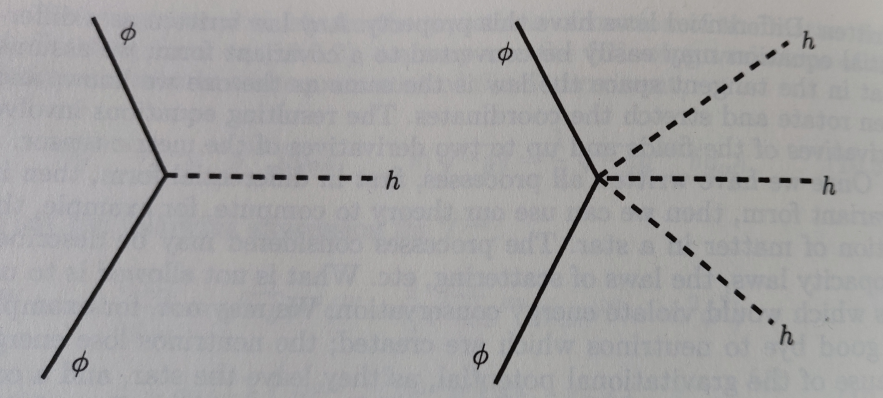
\includegraphics[width=0.7\linewidth]{gfx/feynmanquantumgravity}
	\caption{}
	\label{fig:feynmanquantumgravity}
\end{figure}
In this way, we have arrived at a prescription for calculating quantum mechanical amplitudes for the motion of matter after having started out from a geometrical point of view.\\
In considering the terms in the action, we might consider why the field term might not include a certain proportion $\Lambda$ of $\int \md^4 x \sqrt{-g}$. This would be an integral proportional to the volume of the universe, presumably a constant. The resulting equation for the field behaves somewhat as though the gravitons had a mass and a universal source. The observation of the extremely long range of gravity forces makes it rather pointless to introduce such a term (since mass would imply Yukawa cut-off ?), even though it might lead to a consistent theory. The equations of motion that come from it are
\begin{equation}
G\munu = \Lambda g\munu + \lambda^2 T\munu.
\end{equation}
The constant $\Lambda$ is known as the cosmological constant. Einstein wanted a closed universe, so he assigned to it a value which made steady-state solutions of such a universe possible. This he later referred to as hi Great Mistake; had he chosen it equal to zero, he would have concluded that the unvierse must be expanding (or contracting). 























\newpage
\chapter{Possible Exam problems}
\begin{enumerate}
	\item WAS AN EXERCISE Generalize the Schwarzschild solution for Einstein's equations with a cosmological constant.
	\item PROBABLY Determine the solution representing the spacetime outside a spherically symmetric charged body carrying an electric charge (but no spin and magnetic dipole moment). The sult is the RN sol (c=1) 
	\begin{equation}
		g = - \left(1-\frac{2m}{r} + \frac{\mG e^2}{r^2}\right) \md t^2 + \left(1 - \frac{2m}{r } + \frac{\mG e^2}{r^2}\right)^{-1} \md r^2 + r^2\md \Omega^2,
	\end{equation}
	where $m/\mG$ represents the gravitational mass and $e$ is the electric charge of the body.\\
	Solution: Since fields are static and spherically symmetric we can use for the metric the ansatz of the Schwarzschild solution 
	\begin{equation}
		g=-e^{2 a(r)} \md t^2 + e^{2 b(r)} \md r^2 + r^2\md \Omega^2.
	\end{equation}
	it is again convenient to worj in the orthonormal tetrad 
	\begin{equation}
	\theta^0 = e^a \md t,\; \theta^1= e^b \md r, \; \theta^2 = r \md \vartheta, \; \theta^3 = r\sin\vartheta \md \varphi,
	\end{equation}
	such that the metric then reads:
	\begin{equation}
		g=g\munu \theta^\mu \otimes \theta^\nu, \quad (g\munu) = \mathrm{diag}(-1,1,1,1).
	\end{equation}
	Hence we make the ansatz
	\begin{equation}
		F = \frac{e}{r^2} \theta^0 \wedge \theta^1.
	\end{equation}
	For this the components of the energy-momentum tensor are readily found to be
	\begin{equation}
		T^0_0=T^1_1=-T^2_2=-T^3_3 = -\frac{e^2}{8 \pi r^4},
	\end{equation}
	all other $T\munu =0$. Hence, the equations $G^0_0=8 \pi \mG T^0_0$ and $G^1_1= 8 \pi \mG T^1_1$ become
	\begin{align}
		\frac{1}{r^2} - e^{-2b} \left(\frac{1}{r^2} - \frac{2 b^\prime}{r}\right) &= \frac{\mG e^2}{r^4} \\
		\frac{1}{r^2} - e^{-2b} \left(\frac{1}{r^2} + \frac{2 a^\prime}{r}\right) &= \frac{\mG e^2}{r^4}.
	\end{align}
By subtraction we see that again $a*b=0$. Furthermore, $G_{00}$ equation is equivalent to
\begin{equation}
	(r e^{-2b})^\prime = 1 - \frac{e^2 \mG}{r^2}.
\end{equation}
The metric functions are thus given by
\begin{equation}
	e^{2a} = e^{-2b} = 1 - \frac{2m}{r} + \frac{e^2 \mG}{r^2},
\end{equation}
where $m$ has the same interpretation as for the Schwarzschild solution. The other components of Einstein's equation are also satisfied. It remains to show that Maxwell's vacuum equations are also fulfilled. For this we first note that $F=\md A$, $A=\frac{e}{r} \md t$, hence $\md F=0$. Since $*F=-\frac{e}{r^2} \theta^2 \wedge \theta^3=\md (e \cos \vartheta \md \varphi)$, we have also $\md * F =0$. For later use we write the result in the form
\begin{align}
	g &= - \frac{\Delta}{r^2} \md t^2 + \frac{r^2}{\Delta} \md r^2 + r^2 \md \Omega^2 \\
	F&= - \frac{e}{r^2} \md t \wedge \md r,\\
	\Delta &= r^2 - 2mr + e^2 \mG.
\end{align}
	

\item Show that the effective potential of the Schwarzschild solution has the following properties
\begin{enumerate}
	\item For $L/m < 2 \sqrt{3}$ any incoming particle falls toward $r=2m$
	\item The most tightly bound, stable circular orbit is at $r=6m$ with $L/m=2 \sqrt{3}$ and has fractional binding energy of $1-\sqrt{8/9}$.
	\item Any particle with $E\geq 1$ will be pulled into $r=2m$ if $2\sqrt{3} < L/m < 4$.
\end{enumerate}
\item Redshift Schwarzshild bh p 202 ff ?
\item Show that the Newtonian-limit metric gives the correct deflection of light rays
\item Show that the Newtonian-limit metric gives $4/3$ times the Einstein value for the perihelion precession. This demonstrates once more that the precession of the perihelion is sensitive to non-linearities in GR.
\item Maybe a gravitational waves exercise, even though never did any ?
\item 
\end{enumerate}








1 








\chapter{Important equations of GR - TO DO}
\section{Differential Geomtetry}

\section{Statements from problem sheets}
\begin{enumerate}
\item Euler-Lagrange Equations for field $\phi$
\begin{equation}
	\partial_\lambda \left[\frac{\partial \mL}{\partial(\partial_\lambda \phi)}\right] - \frac{\partial \mL}{\partial \phi} =0.
\end{equation}
For a coordinate $x^\mu$
\begin{equation}
	\frac{\md}{\md \tau} \left(\frac{\partial \mL}{\partial \dot{x}^\mu}\right) - \frac{\partial \mL}{\partial x^\mu}=0.
\end{equation}
\item Null geodesics remain null geodesics $\dot{x}^\mu \dot{x}_\mu=0$ under conformal transformation
\begin{equation}
	g \mapsto \tilde{g} = e^{2 \phi(x^\nu) } g.
\end{equation}
\item On the $S^2$ sphere, one can define forms as on every manifold. With the differential operator of codifferential and hodge-dual, one can then define a divergence or gradient on the sphere. These relations are useful in the
context of spherically symmetric solutions of Einstein’s field equations (e.g. the Schwarzschild
solution). As will be seen in the lecture, the manifold describing space-time can then be foliated
as $M^4 = M^2 × S^2$ . Operators (like the covariant divergence or the Laplacian) on the second
submanifold can be expressed elegantly by differential forms on $S^2$.
\item Note that the following expansion is independent of the metric
\begin{equation}
	\partial_\alpha \phi \partial^\alpha \phi = \partial_0 \phi \partial^0 \phi + \partial_i \phi \partial^i \phi.
\end{equation}
Only upon pulling down the index do we get metric factors in front.
\item For computations of lifetimes, distances and what not for observer near BH, use eom derived from Lagrangian, i.e. try to use the eom
\begin{equation}
	\left(\frac{\md r}{\md \tau}\right)^2 + V(r) = E^2,
\end{equation}
or the conserved quantities 
\begin{equation}
	\langle \dot{\gamma} , \partial_t\rangle = E= const. \qquad \langle \dot{\gamma},\partial_\varphi\rangle = L =const.
	\end{equation}

\item Use integration trick for integral
\begin{equation}
	\md \tau = \int_0^{2m} \frac{\md r}{\sqrt{\frac{2m}{r} -1}}
\end{equation}
thus
\begin{equation}
	r = m(1+\cos \eta),\qquad \md r = - m \sin \eta \md \eta.
\end{equation}
\item radial infall $\Rightarrow$ $\dot{\varphi}=0 \Rightarrow L=0$.
\end{enumerate}
\section{Statements to incorporate}
\begin{enumerate}
	\item The
	appearance of an effective cosmological constant makes it
	impossible to find any solutions of the Einstein field equations in which $g\munu$ is the constant Minkowski  $\eta\munu$. That is, the original symmetry of general covariance,
	which is always broken by the appearance of any given
	metric $g\munu$
	cannot, without fine-tuning, be broken in
	such a way as to preserve the subgroup of space-time
	translations.
\end{enumerate}